\section{Systematics and expected sensitivity}
(outline by David)

\subsection{Systematics: unchanged}What is the same as Run 1-2-3 analysis: few sentences + reference past note.
\subsection{Systematics: What's new}
\subsubsection{GENIE FSI bug-fix} A few validation plots, e.g. Chris' validation work of GENIE weights.
\subsubsection{EXT smoothing} (Alex, in progress)
\label{sec:ext_smoothing}
At the final level of the event selection, the number of EXT events is much too small to reliably produce a non-zero bin count in the analysis histograms. In the previous round of the analysis, an error of 1.4 events was assigned to any bin without any EXT events. This number was derived as the expected error given a uniform prior distribution between 0 and 1 on the expectation value. However, this error assignment could lead to an overly conservative error estimate. For this round, we instead use a KDE to produce a smoothed histogram and calculate the covariance matrix of the smoothed histogram using a bootstrapping technique.

The procedure to produce a smoothed histogram is as follows:
\begin{enumerate}
    \item Fit a gaussian KDE to the data. The bandwidth is automatically chosen using the Silverman's rule. 
    \item For every bin in the histogram, numerically integrate the KDE over the bin range and multiply by the sum of all weights in the sample to produce the expected number of events in that bin. This results in the central value of the histogram.
    \item Repeat steps 1 and 2 100 times using bootstrap samples of the data, but use the same bandwidth as was used to compute the central value. The bootstrap samples are generated by multiplying the weight of every event with a random number drawn from a Poisson distribution with an expectation value of one.
    \item Calculate the covariance matrix of the 100 histograms produced in step 3. This is the covariance matrix of the smoothed histogram.
\end{enumerate}
One issue with this procedure is that the KDE may produce unexpected results when a variable is bounded. For example, the distribution of the cosine of an angle is bounded between -1 and 1 and may be peaked close to one in the case of forward scattering. The KDE would over-smooth this distribution and underestimate the total number of events in the histogram, because it assigns a non-zero probability to values larger than one, which is unphysical. To solve this problem, we use a transformed KDE (TKDE) with a transformation that maps the observed data to the real numbers. For two-sided bounded variables, we use the logit transformation, which is given by $y  = \log\left(\frac{x}{1-x}\right)$, which is applied after first scaling the samples such that the bounds are at 0 and 1. For one-sided bounded variables, first shift (and flip in the case of an upper bound) the data such that the bound is at zero and use the log transformation, $y =  \log(x)$. The Gaussian KDE is then fit to the transformed data, $y$. The probability density is then estimated in the original bounded space using the change of variables formula, $p(x) = p(y)\left|\frac{dy}{dx}\right|$. The covariance matrix is then calculated using the same procedure as above. We demonstrate the effect of the TKDE on the EXT histogram in Fig.~\ref{fig:EXT_smoothing}. The left plot shows the 1D distribution of the cosine of the angle between the track and shower, where the bounded KDE smoothing has been applied to the EXT histogram. The right plot shows the unsmoothed EXT histogram and the two KDE smoothed histograms, one using the bounded KDE and one using the standard KDE. The unbounded KDE misses the peak of the distribution close to one, while the bounded KDE gives a more reasonable estimate.
\begin{figure}
    \centering
    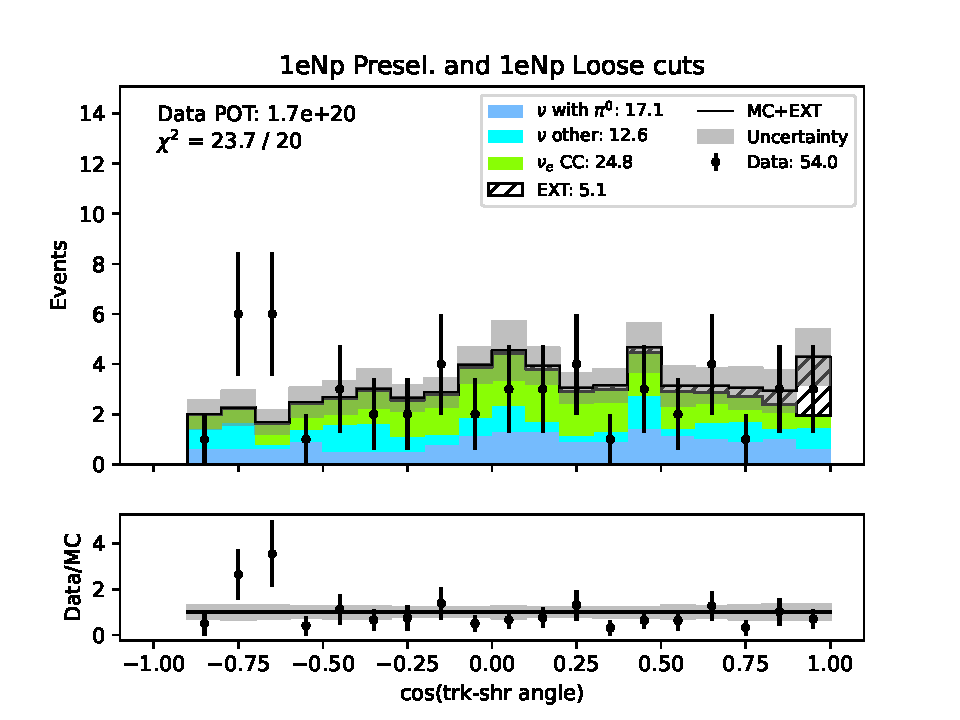
\includegraphics[width=0.45\textwidth]{technote/SystematicsSensitivity/Figures/tksh_angle_NPL_NP_smoothed.pdf}
    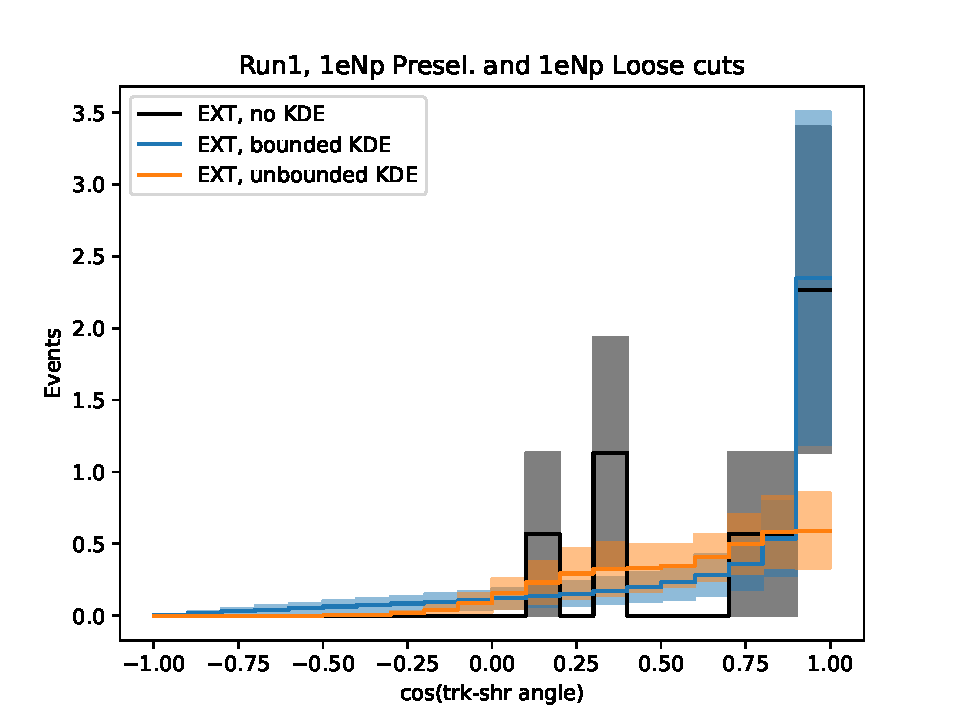
\includegraphics[width=0.45\textwidth]{technote/SystematicsSensitivity/Figures/tksh_angle_NPL_NP_kde_comparison}
    \caption{Comparison of EXT smoothing methods. Left: 1D distribution of the cosine of the angle between the track and shower, where the bounded KDE smoothing has been applied to the EXT histogram. Right: unsmoothed EXT histogram and the two KDE smoothed histograms, one using the bounded KDE and one using the standard KDE.}
    \label{fig:EXT_smoothing}
\end{figure}
Which boundary treatment to use for each variable is decided automatically unless explicitly overridden by the user by the following procedure:
\begin{itemize}
    \item If there are fewer than 5 samples, use the standard KDE.
    \item If all samples fall within the bounds of the binning of the variable, the two-sided bounded KDE is used.
    \item If there are samples above the upper bound and below the lower bound, the standard KDE is used.
    \item If any samples fall above (below) the upper (lower) bound, the one-sided bounded KDE is used.
\end{itemize}
Other special cases to consider are those where only one or no sample at all. In the case of only one sample, we use the standard KDE and set the kernel bandwidth equal to the bin width. If there are no samples at all, we treat the histogram as being empty and the errors to zero\todo{Should we set non-zero errors in this case?}.

\subsubsection{DetVar systematics} Are we assuming Run123 detvars for Run 1-5? Probably true for first sensitivites. \\
Include a table which lists MC stats available on DetVar samples.
\subsubsection{Signal model systematics}

\subsection{systematics summary}

The total systematics error budget is shown in the table of Fig.~\ref{fig:systematicsbudget}.

\begin{center}
\begin{figure}[h]
    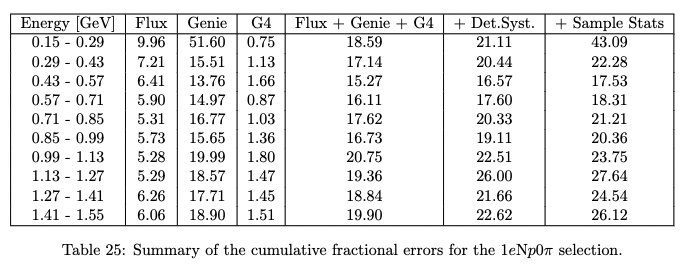
\includegraphics[width=1.00\textwidth]{technote/SystematicsSensitivity/Figures/systematicsbudget.png}
    \caption{Enu spectrum before/after constraint.}
    \label{fig:systematicsbudget}
\end{figure}
\end{center}

\newpage
\subsection{Constraints}
Describe briefly, refer to older analysis.

Show spectrum of nues before and after constraint. See Fig.~\ref{fig:constraint}.

\begin{center}
\begin{figure}[h]
    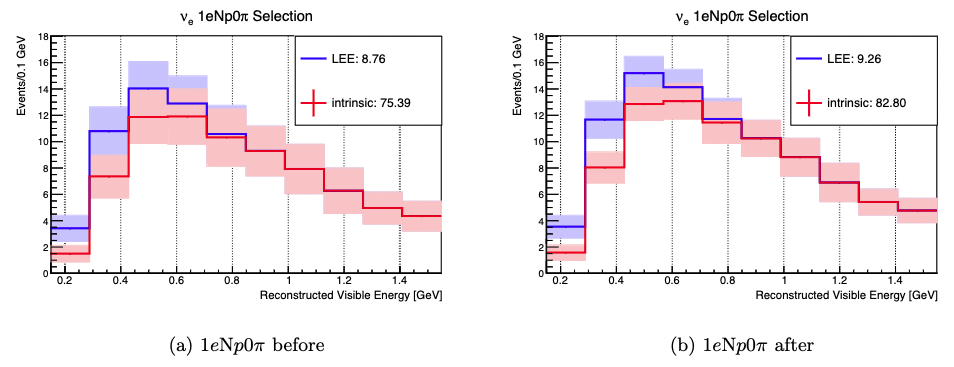
\includegraphics[width=1.00\textwidth]{technote/SystematicsSensitivity/Figures/constraint.png}
    \caption{Neutrino energy spectrum before/after constraint.}
    \label{fig:constraint}
\end{figure}
\end{center}

Show quantitative predicted events and uncertainty (including reduction in uncertainty) before/after constraint. See Table of Fig.~\ref{fig:constrainttable}.

\begin{center}
\begin{figure}
    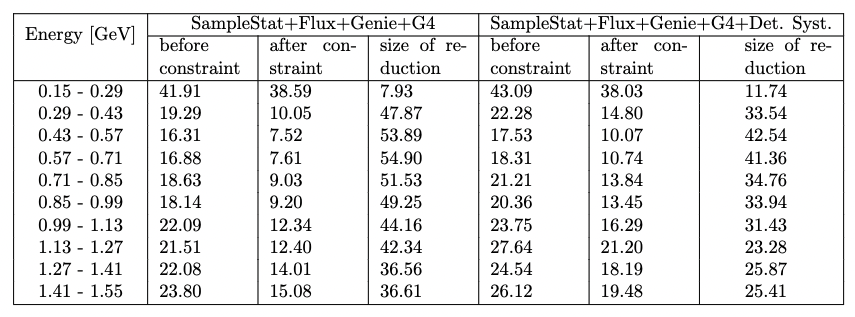
\includegraphics[width=1.00\textwidth]{technote/SystematicsSensitivity/Figures/constrainttable.png}
    \caption{Impact of constraint.}
    \label{fig:constraint} 
\end{figure}
\end{center}

Potentially think of new ideas here

\newpage
\subsection{Sensitivity}
\label{sec:sensitivity}

\subsubsection{Simple Hypothesis Test}

Distribution of test statistic for backgronud-only and signal models, with extracted median sensitivity. See. Fig.~\ref{fig:simplehypothesis}.

\begin{center}
\begin{figure}[h]
    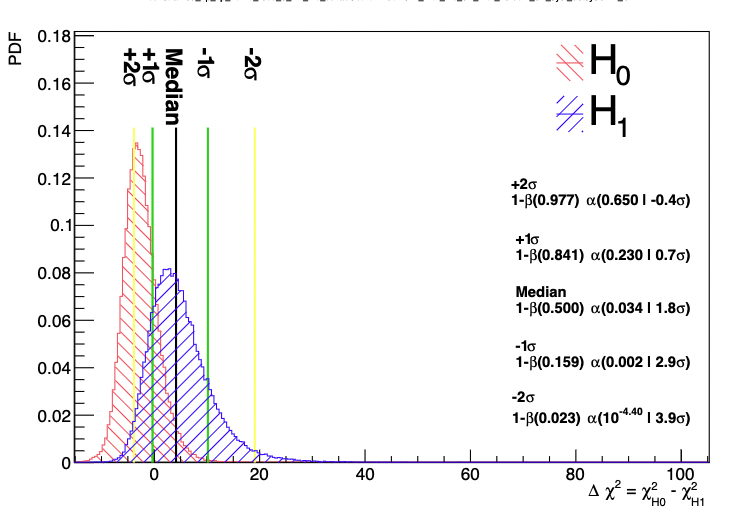
\includegraphics[width=1.00\textwidth]{technote/SystematicsSensitivity/Figures/simplehypothesis.png}
    \caption{Impact of constraint.}
    \label{fig:simplehypothesis} 
\end{figure}
\end{center}

Fig.~\ref{fig:simplehypothesisresults} shows the expected sensitivity for the simple hypothesis test.

\begin{center}
\begin{figure}[h]
    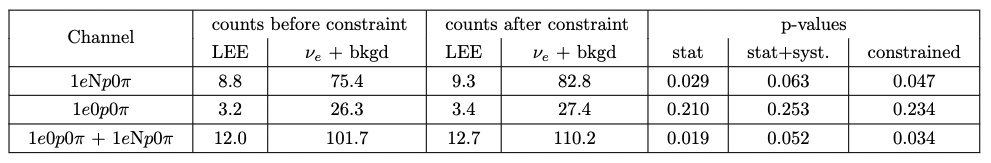
\includegraphics[width=1.00\textwidth]{technote/SystematicsSensitivity/Figures/simplehypothesisresults.png}
    \caption{Impact of constraint.}
    \label{fig:simplehypothesisresults} 
\end{figure}
\end{center}

\newpage
\subsubsection{Signal strength fit}

The signal strength sensitivity results are shown in Fig.~\ref{fig:signalstrengthsensitivity}.
\begin{center}
\begin{figure}[h]
    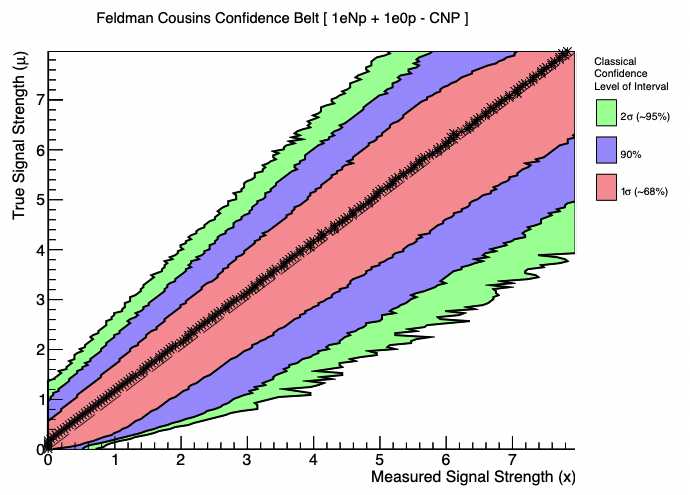
\includegraphics[width=1.00\textwidth]{technote/SystematicsSensitivity/Figures/signalstrengthsensitivity.png}
    \caption{Impact of constraint.}
    \label{fig:signalstrengthsensitivity} 
\end{figure}
\end{center}

\newpage
\subsubsection{Validation of sensitivity vs. SBNFit benchmark}
